\documentclass{rapport}
\usepackage{lipsum}
\usepackage{gensymb}
\usepackage{float}
\usepackage{graphicx} % Required for inserting images
\usepackage{subcaption}
%\usepackage[demo]{graphicx}
\usepackage{tikz,pgfplots}
\usepackage{amsmath, bm, amssymb,amsfonts,amsthm}
\usepackage{float}
\usepackage[version=4]{mhchem}
\usepackage{siunitx}
\usepackage{longtable,tabularx}
\usepackage{makecell}
\usepackage[labelfont=bf]{caption}
 \usepackage{setspace}
\usepackage[table]{xcolor}
\usepackage[x11names,dvipsnames,table]{xcolor} %for use in color links
\usepackage{colortbl}
\usepackage[utf8]{inputenc}
\usepackage{fontspec}
\usepackage{listings}
\usepackage{xcolor}
\usepackage{booktabs} 

% MATLAB style for listings
\definecolor{darkgreen}{rgb}{0,0.5,0}
\lstset{
  language=Matlab,
  basicstyle=\ttfamily\footnotesize,
  keywordstyle=\color{blue},
  commentstyle=\color{darkgreen},
  stringstyle=\color{red},
  numbers=left,
  numberstyle=\tiny\color{gray},
  stepnumber=1,
  numbersep=5pt,
  backgroundcolor=\color{lightgray!20},
  showspaces=false,
  showstringspaces=false,
  tabsize=4,
  captionpos=b,
  breaklines=true,
  breakatwhitespace=false,
  frame=single
}
% Set font as Calibri
\setmainfont{Carlito}[
    Path=./Carlito/,
    Extension = .ttf,
    UprightFont=*-Regular,
    BoldFont=*-Bold,
    ItalicFont=*-Italic,
    BoldItalicFont=*-BoldItalic
    ]
\title{file title} %title of the file


\begin{document}
%----------- Report information ---------

\logo{Images/logos/nus_logo_full-vertical.jpg}
\uni{\textbf{National University of Singapore\\
EE5114: Autonomous Robot Navigation}}
\ttitle{Implementing Simultaneous Localization and Mapping via a Particle Filter (FastSLAM)\\
} %title of the file
\subject{EE5114: Autonomous Robot Navigation} % Subject name

\professor{Dr. Fei \textsc{WANG}} % information related to the professor

\students{Parthiv Vinubhai Kukadia \textsc{(A0304932J)}} % information related to the students

%----------- Init -------------------
        
\buildmargins % display margins
\buildcover % create the front cover of the document

%------------ Report body ----------------

\section{Introduction}
\label{Introduction}
This paper will describe the implementation of Simultaneous Localization and Mapping using a FastSLAM algorithm, which implements a particle filter-based approach. This method allows the UAV to estimate its location while also building a map of the environment at the same time, a crucial aspect of autonomous navigation. This method allows the UAV to be put into any unknown environment and operate in a stable and controlled manner while providing a map of the environment it is in. The algorithm utilized motion estimation, landmark detection, the use of a Kalman filter to update state estimations, and resampling of particles based on their weights. The paper will explain the steps that are undertaken to implement a FastSLAM algorithm, including the theory for motion prediction, the steps required for data association using the Mahalanobis distance, how to mitigate/account for noise in sensor measurements and motion, and ensuring the most accurate estimate of your states while implementing the Kalman filter. It will further highlight the importance of using constraints for angular and distance measurements to ensure a consistent and reliable system without facing any numerical instability issues. The nomenclature used in the report can be found in section 2, and the implementation of FastSLAM can be shown to be broken down in section 3.


\section{Nomenclature}
\label{Nomenclature}
\begin{table}[h!]
\centering
\begin{tabular}{>{\raggedright\arraybackslash}p{8cm} p{8cm}}
\midrule
P = Set of feature points in the 1st frame (x,y) & Q = Set of feature points in the 2nd frame (x,y) \\
SVD = Singular Value Decomposition & d = Determinant of rotation matrix \\
R = Rotation matrix for motion estimation & T = Translation vector for motion estimation \\
$D_{M}(x,\mu)$ = Mahalanobis distance & $\nu$ = Innovation vector \\
K = Kalman gain & $\theta$ = Heading angle (radians) \\
$d_k$ = Perpendicular distance from a point to a line & m = slope/gradient of a line \\
c = Y-intercept of line & $\hat{x}$ = Estimated state vector \\
$\Sigma$ = Covariance matrix of a distribution & $P_{new}$ = Covariance Matrix (new)\\
\bottomrule
\end{tabular}
\end{table}

\pagebreak
\section{Implementing FastSLAM}
\label{Motion_estimation}
The following section covers the 6 different parts edited in implementing FastSLAM via a Particle Filter for the UAV. The sections are titled the name of the Matlab script file, and they will include the code that was filled in, the theory behind the code, and the mathematical equations/formulas used to develop the code.
\subsection{motion estimation.m}
\textbf{Please explain your filled-in code with a snapshot of those lines of code. List formulas you have used for that part of code.}\\
The code provided in Fig. (\ref{fig:MotionEst.}) is used for motion prediction and proposal generation. The code is calculating a rigid-body transformation between the two feature points, P and Q, in their respective frames (2 different frames). The steps undertaken can be shown below:
\begin{enumerate}
    \item Extracting the x-y coordinates of P and Q feature points, where a feature point can be understood as a landmark in an environment and can be used for tasks like motion estimation or object recognition to provide properties of a scene
    \begin{align*}
        P_x &= P(:,1) \\
        P_y &= P(:,2) \\
        Q_x &= Q(:,1) \\
        Q_y &= Q(:,2)
    \end{align*}
    \begin{enumerate}
        \item P and Q are existing matrices defined in the code above representing matched feature points in two frames, where P and Q are [n x 2] matrices.  
        \item P contains the feature points in the first frame, and Q contains the feature points in the second frame
        \item $P_x$, $P_y$ extract the x and y coordinates from the first frame, while $Q_x$ and $Q_y$ extract the x and y coordinates from the second frame
    \end{enumerate}
    \item Calculating the Centroid (mean) of the feature points for both frames
    \begin{align}
        \bar{P} &= \left[ \bar{P}_x, \bar{P}_y \right] \\
        \bar{Q} &= \left[ \bar{Q}_x, \bar{Q}_y \right]
    \end{align}
    \begin{enumerate}
        \item The centroid represents the "mean" position of the points in each set, P and Q
        \item We calculate the mean of the x and y coordinates of both the P and Q feature points and create a variable to store those values, which are required in the next step
    \end{enumerate}
    \item Required to center the points around the centroid
    \begin{align}
        \text{Matrix P} &= \begin{bmatrix}
            P_1 - \bar{P}, P_2 - \bar{P}, P_3 - \bar{P}, ..., P_{max} - \bar{P}
        \end{bmatrix} \\
        \text{Matrix Q} &= \begin{bmatrix}
            Q_1 - \bar{Q}, Q_2 - \bar{Q}, Q_3 - \bar{Q}, ..., Q_{max} - \bar{Q}
        \end{bmatrix}
    \end{align}
    \begin{enumerate}
        \item Since the feature-points are defined using absolute position, we center them around the centroid to obtain relative positions such that the points are then centered around the origin of (0,0) and the feature points are moved from being mean-centered to origin centered.
        \item This is done to eliminate bias, where centering the points around the centroid will help in eliminating any influence the absolute position of points have, and focuses on relative position of the points with respect to the centroid location.
        \item The numerical stability is greater when you center points around the centroid allowing for better calculations when doing singular value decomposition, as we will do next.
    \end{enumerate}
    \item Conduct Singular Value Decomposition (SVD)
    \begin{align}
        [U, S, V] &= \text{svd}(\text{Matrix P} \cdot \text{Matrix Q}^T)
    \end{align}
    \begin{enumerate}
        \item SVD is performed on the centered point matrix of P and Q that was obtained in the previous step.
        \item The decomposition will help in calculating the optimal rotation required between the two point sets P(i) and Q(i).
        \item SVD provides us 3 matrices, U, S, V, which are the decomposed matrices used for estimating the rotation matrix without inducing much noise and in a more  stable manner
    \end{enumerate}
    \item Correction of determinant sign to ensure a proper rotation matrix (R)
    \begin{align}
        d &= \text{sign}(\text{det}(V \cdot U^T))
    \end{align}
    \begin{enumerate}
        \item det($V$ $\cdot$ $U^T$) computes the determinant, where if the determinant is +1 it is a proper rotation matrix, and a determinant of -1 would be a reflection
        \item The value of d corrects the sign of the determinant to make sure that the transformation is not a reflection and is a rotation
    \end{enumerate}
    \item Calculate the Rotation Matrix
    \begin{align}
        R &= V \cdot \begin{bmatrix}
            1 & 0 \\
            0 & d
        \end{bmatrix} \cdot U^T
    \end{align}
    \begin{enumerate}
        \item Calculate the rotation matrix using the results from SVD, ensuring that the determinant of R is 1 to preserve the rotation orientation
    \end{enumerate}
    \item Calculate the Translation vector (T)
    \begin{align}
        T &= R \cdot \bar{P} - \bar{Q}
    \end{align}
    \begin{enumerate}
        \item Calculated by applying the rotation, R, to the centroid of P, - the centroid of Q, providing the translation to alin the two feature sets
        \item We are able to obtain the offset between the two centroids obtained from the two feature points, P and Q
    \end{enumerate}
    \item Extract the Angle of Rotation and Translation
    \begin{align}
        \bar{c}_t &= -atan2\left(R(2), R(1)\right) \\
        [\Delta\bar{x}_t, \Delta\bar{y}_t] &= [T(1), T(2)]
    \end{align}
    \begin{enumerate}
        \item Rotation angle $\theta$ (rads) is obtained from R using eq. (9)
        \item The translation is provided from the vector T
    \end{enumerate}
\end{enumerate}

\begin{lstlisting}
if (assoc_count >= 2)
        % Missing codes start here ...
        
   		% Use matched corners to calculate rotation and translation between
   		% the two frames, (from slide 40 of lecture 4)
        
        % From P and Q, obtain the matched corner x-y coordinates
        P_x = P(:,1); % x is 1st column
        P_y = P(:,2); % y is 2nd column
        Q_x = Q(:,1);
        Q_y = Q(:,2);

        % Calculate the centroid of the feature points for both frames
        mean_P = [mean(P_x), mean(P_y)]; % Centroid of feature point P
        mean_Q = [mean(Q_x), mean(Q_y)]; % Centroid of feature point Q

        % Form Matrix P = [P_1 - mean_P, P_2 - mean_P,... P_max - mean_P]
        Matrix_P = [P_x - mean_P(1), P_y - mean_P(2)];
        % Form Matrix Q = [Q_1 - mean_Q, Q_2 - mean_Q,... Q_max - mean_Q]
        Matrix_Q = [Q_x - mean_Q(1), Q_y - mean_Q(2)];

        % Use Singular Value Decomposition (SVD) to handle uncertainty and
        % noise in seneor measurements
        [U,S,V] = svd(Matrix_P' * Matrix_Q);
        d = sign(det(V * U'));

        % Calculate R, the Rotation matrix
        R = V * [1 0; 0 d] * U';

        % Calculate T, the Translation vector
        T = (R * mean_P') - mean_Q';

        % Motion estimate update step
        theta = -atan2(R(2,1), R(1,1));
        translation = T;

        % Missing codes end here ...
%% Result plotting
path = zeros(4, size(motion_estimate, 2));

for i = 1:size(motion_estimate, 2)
    path(1,i) = motion_estimate(i).x;
    path(2,i) = motion_estimate(i).y;
    path(3,i) = motion_estimate(i).theta;
    path(4,i) = motion_estimate(i).point_count;
end

figure;
labels = {'Motion estimate (x)', 'Motion estimate (y)', 'Motion estimate (\theta)', 'Motion estimate (point count)'};

for i = 1:4
    subplot(4, 1, i);
    plot(path(i, :), 'b*'); 
    ylabel(labels{i}); % Label the y-axis for each subplot
    xlabel('Time (s)');    % Label the x-axis as time for each subplot
end
\end{lstlisting}
\captionof{figure}{MATLAB Code for Motion Estimation}
\label{fig:MotionEst.}
\\
The motion estimation plot can be seen in Fig (\ref{fig:MotionEstimation}), which shows how the motion estimate of the x, and y axes are moving over time, and the motion estimate of theta and the count of points used in localizing and mapping the system. \\
\begin{figure}[H]
  \centering
 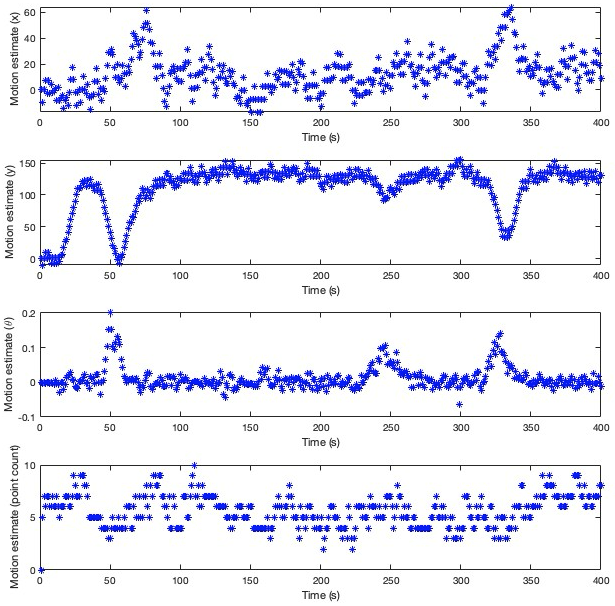
\includegraphics[width=0.8\linewidth, height=0.7\linewidth]{FastSLAM/Motion_Estimate.png}  
\caption{Motion Estimation Chart Over Time}
\label{fig:MotionEstimation}
\end{figure}
The motion path can be seen through Fig (\ref{fig:MotionPath}), which shows how the system is moving around and the map of the area it is moving around. \\
\begin{figure}[H]
  \centering
 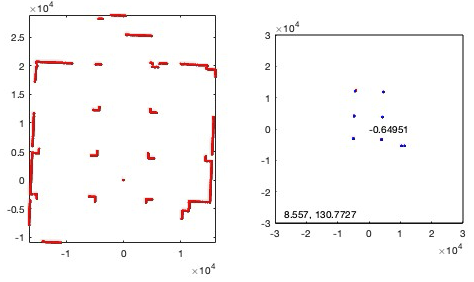
\includegraphics[width=0.7\linewidth, height=0.5\linewidth]{FastSLAM/Motion_Path.png}  
\caption{Actual Motion Path vs. Localized Estimated Path}
\label{fig:MotionPath}
\end{figure}

\textbf{Please explain what line 51-97  is trying to do?}\\
Lines 51-97 are associating the feature points P and Q based on their Mahalanobis distances. Where the Mahalanobis distance is a measure of the distance between a point and a distribution, taking into account the correlations of the data set and the shape of the distribution. This method allows the identification of corresponding features between P and Q detected corners, ensuring that only unique associations are taken as input while accounting for covariance in the measurements. The mahalanobis distance can be measured as:
\begin{equation}
D_M(\mathbf{x}, \boldsymbol{\mu}) = \sqrt{(\mathbf{x} - \boldsymbol{\mu})^T \Sigma^{-1} (\mathbf{x} - \boldsymbol{\mu})}
\label{EQ:DM}
\end{equation}
Where, \( D_M \): Mahalanobis distance between the point \( \mathbf{x} \) and the mean vector \( \boldsymbol{\mu} \). \( \mathbf{x} \): A point (vector) in the feature space for which the distance is being measured. \( \boldsymbol{\mu} \): Mean vector of the distribution (vector), representing the average position of all points in the dataset. \( \Sigma \): Covariance matrix of the distribution, representing the variance and covariance of the features in the dataset. \( T \): Transpose of the vector. \( \Sigma^{-1} \): Inverse of the covariance matrix.\\

A breakdown of the code can be shown below:
\begin{enumerate}
    \item Check for detected corners: check if there are any corners in 2nd set of corners and 1st set of corners (if either empty, then code block will be skipped)
    \begin{lstlisting}
    if (~isempty(corners2))
        if (~isempty(corners1))
    \end{lstlisting}
    \item Count the detected corners: \# of corners in corners1 and corners2
    \begin{lstlisting}
    known_corners_count = size(corners1, 2);
    detected_corners_count = size(corners2, 2);
    \end{lstlisting}
    \item Create the Mahalanobis distance Matrix: Create the matrix and initialize it to be "threshold" values. As the code iterates through, it will update this matrix with distance between pairs of detected corners
    \begin{lstlisting}
    mahalanobis_matrix = threshold.*ones(detected_corners_count, known_corners_count);
    \end{lstlisting}
    \item Calculate the Mahalanobis Distance: Iterate over each corner pair detected, and for each pair, calculate the difference in x-coordinate, y-coordinate, and angles (using slam in pi.m). Using Eq.(\ref{EQ:DM}) calculate the distance and store it into the matrix created above if it is less than the threshold values.
    \begin{lstlisting}
    for j = 1:detected_corners_count
        for k = 1:known_corners_count
		  % Components of x-mu
		  a = corners2(j).x-corners1(k).x;
		  b = corners2(j).y-corners1(k).y;
		  c = slam_in_pi(corners2(j).angle-corners1(k).angle);

		  mahalanobis_dist = sqrt([a b c] * (covariance^-1) * [a; b; c]);
		  if (mahalanobis_dist < threshold)
            mahalanobis_matrix(j,k) = mahalanobis_dist;
		  end
	   end
    end
    \end{lstlisting}
    \item Associating the points: find minimum distance within the mahalanobis matrix, if these distances are less than the threshold value, an association can be made and it finds the index of that value in the matrix and updates the associated count and stores them in the P and Q matrix. This continues to happen until associations can no longer be made, at which point the loop breaks.
    \begin{lstlisting}
while 1
    mahalanobis_min = min(min(mahalanobis_matrix));
    if (mahalanobis_min < threshold)
		% Associate, add to matrix of points
		[d_index, k_index] = find(mahalanobis_matrix == mahalanobis_min);
					
		if (size(d_index, 1) > 1)
			d_index = d_index(1);
		end
		if (size(k_index, 1) > 1)
			k_index = k_index(1);
		end
					
		assoc_count = assoc_count + 1;
		P(assoc_count,:) = [corners1(k_index).x corners1(k_index).y];
		Q(assoc_count,:) = [corners2(d_index).x corners2(d_index).y];
                    
		% Eliminate row and column from further consideration
		mahalanobis_matrix(d_index,:) = (threshold+1).*ones(1, known_corners_count);
		mahalanobis_matrix(:,k_index) = (threshold+1).*ones(detected_corners_count, 1);
	else
		break;
	end
end
    \end{lstlisting}
\end{enumerate}

\textbf{In the last part of the file (before plotting), what do you think is the advantage of constraining the change of x, y and theta?}\\
Constraining the change of x, y, and $\theta$ has many benefits such as enhancing the stability and accuracy of motion estimates, increasing the robustness of the system, and ensuring smoother trajectories through a less noisy system providing better navigation and mapping.\\

The system is more stable since constrained changes reduce the opportunity to destabilize the robot through fewer abrupt changes, which allows the UAV to navigate in a smoother manner while avoiding obstacles and following objects providing more stable and controlled navigation. \\

The system can provide more accurate motion estimates because the algorithm incorporates the estimated states of angle-pre and translation-pre, which improve the trajectory estimation as it takes into account the previous system state as well. \\

The system is more robust as a result of fewer measurement errors. Constrained values means that the noisy data from sensors from estimated position and orientation can be mitigated, reducing the impact of the errors on the system and providing a more accurate estimate for the system. \\

The UAV is able to achieve a smoother motion by preventing jumps in the position and orientation of the system and limiting changes to be within a specific threshold. This limiting can mitigate the noise or measurements that are outliers to affect the system and help provide a smoother motion estimate.\\

A constraint in the change of x,y, and $\theta$ also enforces smaller adjustments to the system from the sensors, which can reduce the over-corrections or oscillations that may occur in the position and orientation of the UAV due to sudden changes. This will also improve the association between frames through constrained changes, which increases the possibility of correctly matching features when the system is expecting smaller motion.\\

Finally, since the real world has several physical constraints on how quickly a robot can maneuver, we can use constraints to replicate practical scenarios to the best of our abilities and mimic real-world dynamics.

\subsection{slam lidar feat extrn.m}
\textbf{Please explain all your filled-in codes with a snapshot of those lines of code. List formulas you have used for that part of code.}\\
The lines of code filled in were related to vector algebra and geometric properties of line segments. The code starts by identifying the direction vectors of the lines, then normalizing the vectors, calculating the angle between the vectors, filtering based on angle ranges, and finally, computing the heading of the corner. Below, the equations used to calculate angle span of the corner and using corner features to calculate heading direction of the corner will be discussed, with the implemented code to be found in Fig. (\ref{fig:SLAMLidarExTRN.}).
\begin{enumerate}
    \item Define the direction vectors of the lines
    \begin{align}
     \mathbf{v}_1 = \begin{bmatrix} x_2 - x_1 \\ y_2 - y_1 \end{bmatrix}\\
     \mathbf{v}_2 = \begin{bmatrix} x_4 - x_3 \\ y_4 - y_3 \end{bmatrix}
    \end{align}
    \begin{enumerate}
        \item Where (x1,y1) and (x2,y2) for are the start and end points of the first (line(i)), and (x3,y3) and (x4,y4) are the start and end points for the second line (line (i+1)).
        \item These vectors will represent the direction of the two line segments, which will be used to calculate the angle between the two lines
    \end{enumerate}
    \item Calculate the angle between vectors
    \begin{align}
    \theta = \cos^{-1} \left( \frac{\mathbf{v}_1 \cdot \mathbf{v}_2}{\|\mathbf{v}_1\| \|\mathbf{v}_2\|} \right)
    \end{align}
    where,
    \begin{align*}
    \mathbf{v}_1 \cdot \mathbf{v}_2 = (x_2 - x_1)(x_4 - x_3) + (y_2 - y_1)(y_4 - y_3)\\
    \|\mathbf{v}_1\| = \sqrt{(x_2 - x_1)^2 + (y_2 - y_1)^2}\\        \|\mathbf{v}_2\| = \sqrt{(x_4 - x_3)^2 + (y_4 - y_3)^2}
    \end{align*}
    \begin{enumerate}
        \item Angle $\theta$ between the two vectors can be found using the dot product formula
        \item The dot product requires you to find the magnitudes of both vectors, which are the euclidean normals of the vectors 
    \end{enumerate}
    \item Define angle range filter
    \begin{enumerate}
        \item For corners to be valid, the angle should be between 60\degree to 120\degree, but defined in radians since our system is operating in radians.
        \item This filtering condition can help us identify what is a valid corner vs. what is not a valid corner
    \end{enumerate}
    \item Define the heading of the corner
    \begin{align}
    \text{heading} = \text{slam\_in\_pi}\left( \text{atan2}(\text{heading2}, \text{heading1}) + \pi \right)
    \end{align}
    Where, atan2 computes the angle between the vector components heading1 and heading2. Adding $\pi$ shifts the angle by 180 $\degree$. The function \texttt{slam\_in\_pi} ensures that the resulting angle lies within the range [- $\pi$, $\pi$], and heading1 and heading 2 can be calculated using:
    \begin{align*}
    \text{heading1} = \frac{v_1(1)}{\|\mathbf{v}_1\|} + \frac{v_2(1)}{\|\mathbf{v}_2\|}\\
    \text{heading2} = \frac{v_1(2)}{\|\mathbf{v}_1\|} + \frac{v_2(2)}{\|\mathbf{v}_2\|}
    \end{align*}
    \begin{enumerate}
        \item The heading direction of the corner is defined as the average of the angles between the two consecutive lines.
        \item Define heading, using the slam in pi function, providing it our heading inputs for the corner. The function is used to normalize an angle so that it lies within the function range of [$-\pi,\pi$] radians
    \end{enumerate}
\end{enumerate}

\begin{lstlisting}
 % Missing codes start here ...
    % Calculate the direction vector of the two lines
    v1 = [lines(i).p2.x - lines(i).p1.x, lines(i).p2.y - lines(i).p1.y];
    v2 = [lines(i+1).p2.x - lines(i+1).p1.x, lines(i+1).p2.y - lines(i+1).p1.y];

    % Calculate angle span of the corner
    angle = acos(dot(v1/norm(v1),v2/norm(v2))); % Normalize the vectors
                
    % Only use corner features having angle from 60 to 120 degrees 
    if (angle > deg2rad(60) && angle < deg2rad(120))
	% Calculate heading direction of the corner
        heading1 = v1(1)/norm(v1) + v2(1)/norm(v2);
        heading2 = v1(2)/norm(v1) + v2(2)/norm(v2);
        heading = slam_in_pi(atan2(heading2, heading1) + pi);
    % Missing codes end here ...
\end{lstlisting}
\captionof{figure}{MATLAB Code for Slam Lidar feat extrn}
\label{fig:SLAMLidarExTRN.}

\subsection{slam lidar split merge.m}
\textbf{Please explain all your filled-in codes with a snapshot of those lines of code. List formulas you have used for that part of code.}\\
For this part of the code, it is required to find the furthest point to the defined line. Begin by calculating the distance of a set of points from the defined line. Then update the values in the point distances array from the calculation made to calculate the distance of the different points from the line. Finally, find the largest distance of a point to the line by comparing it to the defined "winner value" which is the absolute value of the point distances array. We are provided the initialized values of the distance array, the winner values, and the winner index. The calculations to find the distance of a set of points from a line and finding the point that is furthest from the line can be done using the steps shown below, and the code can be found in Fig (\ref{fig:SLAMLidarMerge.}):\\
\begin{enumerate}
    \item Calculate the perpendicular distance from a point to a line
    \begin{align}
    d_k = \frac{|(x_2 - x_1)(y_1 - y_k) - (x_1 - x_k)(y_2 - y_1)|}{\sqrt{(x_2 - x_1)^2 + (y_2 - y_1)^2}}
    \end{align}
    Where $x_k, y_k$ are the coordinates of the point $P_k$, $x_1, y_1$ and $x_2, y_2$ are the coordinates of the two points defining the line, $d_k$ is the perpendicular distance from point $P_k$ to the line.
    \begin{enumerate}
        \item Calculating the shortest distance of the set of points to the line
        \item This is done in a loop since there are multiple points that require the distance to be calculated for
    \end{enumerate}
    \item Finding the furthest point from the line
    \begin{align*}
        d_k \geq winner value
    \end{align*}
    \begin{enumerate}
        \item Check to see if the current distance of the point is greater than the last furthest distance (winner value)
        \item If the new points distance is greater than the last recorded longest distance, then we update the "winner value" to be that distance and we update the "winner index" to be the current value of k.
    \end{enumerate}
\end{enumerate}

\begin{lstlisting}
% Missing codes start here ...
% Find furthest point to this line 
point_distances = zeros(1, last);
winner_value = abs(point_distances(1));
winner_index = 1;

for k = 1:last
    % Loop over to calculate the distance of the different points from the line
    distances = abs(((x2 - x1) * (y1 - point(k).y) - (x1 - points(k).x) * (y2 - y1)) / sqrt((x2 - x1)^2 + (y2 - y1)^2));
    
    % Update the values in point_distances matrix
    point_distances(k) = distances;

    % Finding the largest distance of a point to the line
    if distances >= winner_value
        winner_value = distances;
        winner_index = k;
    end
end
% Missing codes end here ..
\end{lstlisting}
\captionof{figure}{MATLAB Code for Slam Lidar split merge}
\label{fig:SLAMLidarMerge.}\\

\textbf{Please explain what problem is line 11-40 in the original ‘slam lidar split merge.m’ trying to solve? Why does the solution need to use if/else to consider two cases?}\\
Lines 11-40 is solving finding the equation of a line in 2D space and then finding the angle $\theta$ and distance r related to the line. It is to identify the orientation and distance of the line when it is horizontal vs. vertical. 
\begin{enumerate}
    \item The code is used to calculate the equation of the line when it is more horizontal (|$x_2$ - $x_1$| > |$y_2$ - $y_1$|) and the line is expressed in the form y = mx + c
    \item Else the code is used to calculate the equation of the line when it is more vertical (|$x_2$ - $x_1$| $\leq$ |$y_2$ - $y_1$|) and the line is expressed in the form x = my + c.
    \begin{enumerate}
        \item Horizontal case (y = mx+c), used when the change in x is greater than the change in y, and the gradient can be calculated using m = $\frac{y_2 - y_1}{x_2 - x_1}$, and y-intercept c = $y_1$ - m$x_1$.
        \item Vertical case (x = my+c), used when the change in y is greater than or equal to the change in x, and the gradient can be calculated using m = $\frac{x_2 - x_1}{y_2 - y_1}$, and y-intercept c = $x_1$ - m$y_1$.
    \end{enumerate}
    \item The if/else structure is used to validate the relative magnitude of |$y_2$ - $y_1$| and |$x_2$ - $x_1$| to identify whether the line is actually more horizontal or more vertical, based on the identification, the code will switch between the horizontal or vertical calculation to ensure numerical stability.
    \begin{enumerate}
        \item Numerical stability: For lines where the slope is very steep, instead of expressing the line as y = mx + c, the line is expressed as x = my + c to ensure that the numerical instability is not so large, and the slope is a function of y to avoid large and extreme values
        \item Angle calculation: The calculation is done differently for different orientations. If the line is more horizontal, $\theta$ is $tan^{-1}$(m), the slope, which is adjusted by $\frac{\pi}{2}$ to make sure that it is perpendicular to the line. If the line is more vertical, $\theta$ is adjusted to align properly with the geometry using $\frac{\pi}{2}$, where $\theta$ is ($\frac{\pi}{2}$ - $\theta$).
        \item The distance can be calculated using the absolute value of c (the y-intercept) and cos ($\theta$), where the distance is $c x cos(\theta)$.
    \end{enumerate}
\end{enumerate}
Therefore, the if/else structure allows for better adaptation of the code to various line orientations. This is done to ensure that the calculations are stable and accurate and regardless of the orientation of the line in space, we are able to keep the system stable, mitigating numerical instability.

\subsection{slam resample.m}
\textbf{Please explain all your filled-in codes with a snapshot of those lines of code. List formulas you have used for that part of code.}\\
The code is used to implement a resampling process for a particle filter. Resampling is when the algorithm is used to focus on the particles to understand the current state of the system better utilizing weights of the particles. The higher the weight of the particle, the closer the estimate of current state is to the true state, allowing the system to avoid the lower-weighted particles. The method implemented in Stochastic universal sampling, and the code can be found in Fig (\ref{fig:SLAMresample}). The equations used and theory are described below:
\begin{enumerate}
    \item Generate a random number that is between 0 and the total weight of the particles to determine what particle is to be selected in the resampling process.
    \begin{align*}
        \text{random\_number} \sim \mathcal{U}(0, W_{\text{total}})
    \end{align*}
    \item Calculate the cumulative weight of the particles to match the random number to a specific particle, such that whenever the cumulative weight exceeds the number generated, that particle is selected.
    \begin{align}
        W_{\text{cum}} = \sum_{k=1}^{j} w_k
    \end{align}
    \item Add the selected particle to the new set of particles, such that we reset its weight to the initial weight of all the particles
    \begin{align*}
        w_{\text{new}} = \text{init\_weight}
    \end{align*}
\end{enumerate}

\begin{lstlisting}
% Create an array to store newly resampled particles
new_particles = particles;

for i = 1:particles_count
    % Missing codes start here
    % Generate a number between the total weight and 0
    random_num = rand() * weight_total;

    % Resamples particles based on their weights
    cum_weight = 0;
    for k = 1:particles_count
        cum_weight = cum_weight + particles(k).weight;
        if cum_weight >= random_num
            % Select the following particle to be resamples
            new_particles(i) = particles(k);
            break;
        end
    end

    % Afterwards, each new partical should be given the same init_weight
    new_particles(i).weight = init_weight;

    % Missing codes end here
    end

% Replace the old particles with new ones
particles = new_particles;
\end{lstlisting}
\captionof{figure}{MATLAB Code for Slam resample}
\label{fig:SLAMresample}


\subsection{slam crnr kf.m}
\textbf{Please explain all your filled-in codes with a snapshot of those lines of code. List formulas you have used for that part of code.}\\
The matlab script is implementing a Kalman Filter through estimating the state of a system based on the noisy measurements and reflecting that onto the state estimates. The code iteratively estimates the state using predictions and noise observations and maintains an accurate estimate with uncertainty involved through using the kalman gain and innovation. The code used to completed the implementation of the Kalman Filter can be found in Fig (\ref{fig:SLAMcrnrkf.}). The equations used to complete the code are as follows:
\begin{enumerate}
    \item Updating the State
    \begin{align}
        \hat{x}_{new} = \hat{x}_{old} + K \cdot \nu
    \end{align}
    Where $\hat{x}$ is the estimated state, K is the Kalman Gain, and $\nu$ is the innovation
    \begin{enumerate}
        \item Innovation is the difference in the actual measurement and the predicted from the current state estimate
        \item State estimate will include the position, heading, and angle, and will be the old estimate + some proportion of the innovation (decided by K)
        \item Slam in Pi function was used when updating the mean of the corner's heading and angle because they are angular measurements. The Slam in Pi function is useful in making sure that the angles remain within the specified range.
        \item The implementation of Slam in Pi supports consistency and stability as well as provides a better estimate and update process by constraining the angles to stay within a specific range to avoid numerical instability, maintain measurement consistency, and ensuring that angles are provided in a relative state to the system (e.g., 0 radians instead of 2$\pi$ radians).
    \end{enumerate}
    \item Updating the Covariance
    \begin{align}
        P_{new} = (I - K) P_{old}
    \end{align}
    Where K is the Kalman Gain, I is the Identity matrix, and P is the corner covariance.
    \begin{enumerate}
        \item Uncertainty is reduced in the state estimate with the inclusion of covariance
    \end{enumerate}
\end{enumerate}
\begin{lstlisting}
% Missing codes start here ...
% Update mean of this corner 
known_corner.x = known_corner.x + K(1,1) * innovation(1,1);
known_corner.y = known_corner.y + K(2,2) * innovation(2,1);
known_corner.heading = slam_in_pi(known_corner.heading + K(3,3) * innovation(3,1));
known_corner.angle = slam_in_pi(known_corner.angle + K(4,4) * innovation(4,1));

% Update covariance of this corner
I = eye(size(K));
known_corner.covariance = (I - K) * known_corner.covariance;
% Missing codes end here ...
\end{lstlisting}
\captionof{figure}{MATLAB Code for Slam crnr kf}
\label{fig:SLAMcrnrkf.}


\subsection{slam.m}
\textbf{Please explain all your filled-in codes with a snapshot of those lines of code. List formulas you have used for that part of code.}\\
The code block is used to simulate the motion model of the UAV in the SLAM system by making sure that it updates each particle's position and orientation accounting for noise to ensure that the system takes into account uncertainties in movement. The task requires applying rotation and translation to the particles through the inclusion of noise in the uncertainty calculation within SLAM. Need to update the rotation noise (angle $\theta$) of each particle using some random noise, which includes both additive and proportional noise components (constant noise and proportional noise to current angle). Similarly, need to update the translation noise (position x and y) of each particle using some random noise, which includes both additive and proportional noise components in the x-y direction. The code to implement the rotation and translation noise can be found in Fig (\ref{fig:SLAM}). The equations used to apply rotation and translation can be shown below:
\begin{enumerate}
    \item Begin by updating rotation with noise
    \begin{align}
        \Delta \theta_j = \theta_j \left( 1 + \eta_{\text{rotation}} \right) + \xi_{\text{rotation}}\\
        \theta_j^{\text{new}} = \theta_j + \Delta \theta_j
    \end{align}
    Where, $\eta_{rotation}$ $\sim$ $\mathcal{N}$(0, $\sigma_{\theta,proportion}^2$) is the proportional rotation noise,$\xi_{rotation}$ $\sim$ $\mathcal{N}$(0, $\sigma_{\theta,additive}^2$) is the additive rotation noise.
    \begin{enumerate}
        \item Orientation of each particle is done from the robot's motion estimate, and therefore random noise is added to predict the restoration
        \item Additive noise is used as a fixed value independent of the angle
        \item Proportional noise is used equal to the current angle $\theta$
    \end{enumerate}
    \item Update translation with noise
    \begin{align}
        \Delta x_j = x_j \left( 1 + \eta_{\text{translation},x} \right) + \xi_{\text{translation},x}\\
        \Delta y_j = y_j \left( 1 + \eta_{\text{translation},y} \right) + \xi_{\text{translation},y}
    \end{align}
    Where, $\eta_{translation,x}$ $\sim$ $\mathcal{N}$(0, $\sigma_{x,proportion}^2$) is the proportional noise in the x-direction,  $\eta_{translation,y}$ $\sim$ $\mathcal{N}$(0, $\sigma_{y,proportion}^2$) is the proportional noise in the y-direction, $\xi_{translation,x}$ $\sim$ $\mathcal{N}$(0, $\sigma_{x,additive}^2$) is the additive noise in the x-direction, $\xi_{translation,y}$ $\sim$ $\mathcal{N}$(0, $\sigma_{y,additive}^2$) is the additive noise in the y-direction.
    \begin{enumerate}
        \item The translation of each particle is done through incorporating random noise. The particle is moving in the x-y direction from the estimated translation.
        \item Noise is added to the system to simulate real-world inaccuracies, where additive and proportional components are used for translation noise
        \item Additive noise: a noise that has fixed value to add to the translation
        \item Proportional noise: a noise that have value proportional to the current x-y distance
    \end{enumerate}
    \item Updating position after rotation and translation
    \begin{align}
        x_j^{\text{new}} = x_j + \cos(\theta_j^{\text{new}}) \cdot \Delta x_j - \sin(\theta_j^{\text{new}}) \cdot \Delta y_j\\
        y_j^{\text{new}} = y_j + \sin(\theta_j^{\text{new}}) \cdot \Delta x_j + \cos(\theta_j^{\text{new}}) \cdot \Delta y_j
    \end{align}
    Where $\theta_j^{new}$ is the updated orientation of particle j.
    \begin{enumerate}
        \item In the global frame, apply a rotation to update the new position of the particle using the change in orientation and translation.
        \item The update in position uses the robot's new heading angle ($\theta$) and the translation in noise in the x and y direction.
    \end{enumerate}
\end{enumerate}

\begin{lstlisting}
for j = 1:particles_count		
    % Missing codes start here ...
    % Apply rotation to all particles with (additive and proportional) noises 
    rotation_additive = theta_noise_add * randn(1);
    rotation_proportional = theta_noise_proportion * randn(1);

    % Apply translation to all particles with (additive and proportional) noises 
    translation_additive_x = translation_noise_add * randn(1);
    translation_additive_y = translation_noise_add * randn(1);
    translation_proportion_x = translation_noise_proportion * randn(1);
    translation_proportion_y = translation_noise_proportion * randn(1);
        
    % New orientation and position based on the heading and translation
    delta_theta = (motion_estimate(j).theta * (1 + rotation_proportional)) + rotation_additive;
    delta_x = (motion_estimate(j).x * (1 + translation_proportion_x)) + translation_additive_x;
    delta_y = (motion_estimate(j).y * (1 + translation_proportion_y)) + translation_additive_y;
        
    % Add random rotation and translation noise
    particles(j).theta = particles(j).theta + delta_theta;
    particles(j).x = particles(j).x + (cos(particles(j).theta) * delta_x) - (sin(particles(j).theta) * delta_y);
    particles(j).y = particles(j).y + (sin(particles(j).theta) * delta_x) + (cos(particles(j).theta) * delta_y);

    % Missing codes end here ...
\end{lstlisting}
\captionof{figure}{MATLAB Code for SLAM}
\label{fig:SLAM}
\\
Running the SLAM file provides an output that shows the localization and the mapping performed by the UAV. The video can be found in the .zip file labeled "slam.mp4". A still image of the simulation can be seen below in Fig (\ref{fig:SLAMSim}). The Still image shows how the algorithm can identify the different corners using our implemented method and successfully maneuver within the enclosed environment. The slam.mp4 file will show how accurately the system is able to operate in the enclosed area showing a successful implementation of SLAM via a Particle Filter.\\
\begin{figure}[H]
  \centering
 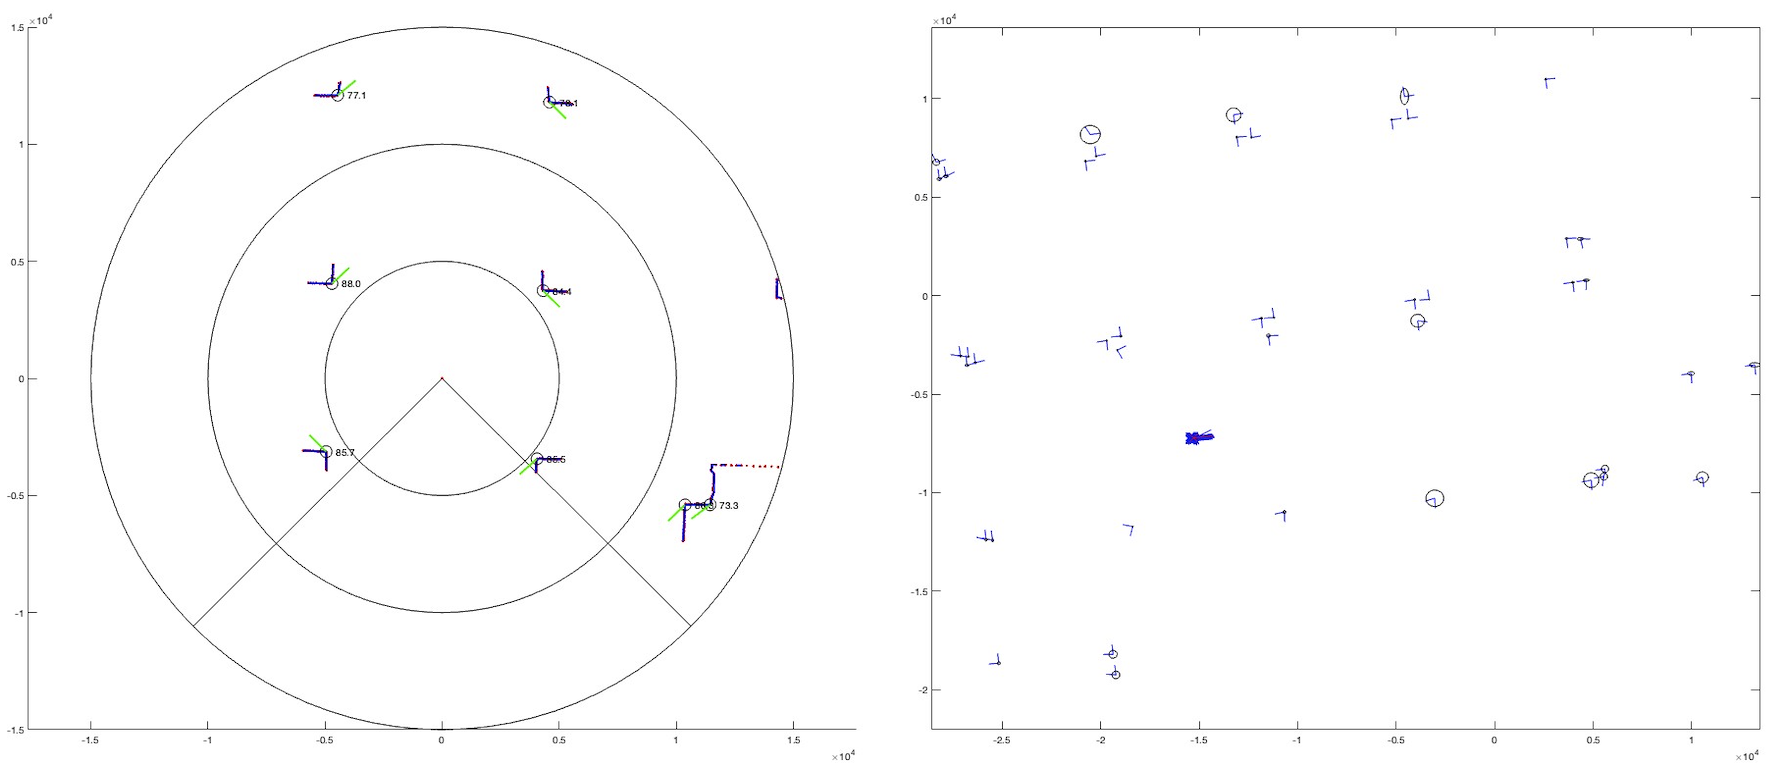
\includegraphics[width=1\linewidth, height=0.7\linewidth]{FastSLAM/SLAMsim.png}  
\caption{Simulation of Localization and Mapping using SLAM via Particle Filter}
\label{fig:SLAMSim}
\end{figure}

\subsection{slam in pi.m}
\textbf{Please explain what ‘slam in pi.m’ function is trying to achieve.}\\
The function is used for angular measurements to ensure that they are bounded/constrained within the specified ranges. Using this function helps the implementation of SLAM by making sure that the angular values are accurate and their is no numerical instability occurring throughout the calculations in SLAM by making the angular values consistent (e.g., 0 radians instead of 2$\pi$ radians). The smaller the values are, the easier it is for the SLAM algorithms to compute at a higher accuracy and avoid any jumping in values to cause instability in the simulated system. In our case, we are restricting the angles to be within the range of [-$\pi$,$\pi$], which will help our system in mitigating errors related to state estimations from inconsistent trigonometric calculations and will support the mapping process that we are using through SLAM. We tackle the 5 major issues using the slam in pi function:
\begin{enumerate}
    \item Eliminate the periodic nature of angles, where the function ensures that the value of the angular measurements will stay within the given range, and not provide values like -2$\pi$, when the value can be 0.
    \item Normalize angles to maintain a consistent range of angles for calculations, such that the angles are all within the provided range when doing geometric transformations to avoid misinterpretation of orientation and position of points in the environment.
    \item Avoid misinterpretation of data through normalizing angles so that when Kalman Filter is used in SLAM, the integration of multiple measurements and states are all in the same physical direction represented in the same way.
    \item Ensure a stable system by allowing the algorithm to operate robustly having consistent angles bounded within a given range, which inturn improves the stability of the system and provides a better performance in real-time
    \item Prevent causing errors in the SLAM algorithm by normalizing the angles to avoid divergence in the algorithm or producing inaccurate maps or localization due to higher/greater angular estimates.
\end{enumerate}\\

\textbf{Where are the locations this function is called. Why are they necessary?}\\
Since the benefits of using the slam in Pi function can be seen and since we know their necessity, it has been implemented in a number of locations throughout our implementation of SLAM. We have used the Slam in Pi Function in 17 locations across all the matlab scripts:
\begin{enumerate}
    \item motion estimation.m
    \begin{enumerate}
        \item To calculate mahalanobis distance: Function used to handle the angular difference when calculating the distance, ensuring a normalized angular difference, ensuring the distance calculations accurately reflect true orientation difference, and to maintain a robust SLAM algorithm by handling angular wrap-around to support localization and feature matching
        \begin{lstlisting}
            % Components of x-mu
		a = corners2(j).x-corners1(k).x;
		b = corners2(j).y-corners1(k).y;
		c = slam_in_pi(corners2(j).angle-corners1(k).angle);
        \end{lstlisting}
        \item Constraining theta change to be within a threshold: Function used to ensure smooth motion by avoiding any rapid changes in orientation, making sure that there is a consistent state estimate by having normalized angles, and adjusting the angles before using them in SLAM calculations for the robot's movement.
        \begin{lstlisting}
        % Constrain theta change to be within a threshold
        if (slam_in_pi(theta - theta_pre) > 0.05)
            theta = theta_pre + 0.05;
        elseif (slam_in_pi(theta - theta_pre) < -0.05)
            theta = theta_pre - 0.05;
        end
        theta = slam_in_pi(theta);  
        \end{lstlisting}
    \end{enumerate}
    \item slam lidar split merge.m
    \begin{enumerate}
        \item Used to define theta: Function used to define theta for horizontal and vertical line if/else statement, to ensure that the calculations have normalized angles to ensure calculations are stable and accurate, which supports keeping the system stable regardless of the orientation of the line, mitigating numerical instability.
    \end{enumerate}
    \item slam lidar feat extrn.m
    \begin{enumerate}
        \item Calculate heading direction of the corner: Function used in constraining the heading direction of a corner feature to ensure that it is within the valid range of angles. This will support normalizing computed heading angles to stay in our calculation range, it will mitigate larger angles being recorded, and ensure that the heading angle is adjusted before being taken into consideration for trigonometric functions to ensure consistency
        \begin{lstlisting}
	% Calculate heading direction of the corner
        heading1 = v1(1)/norm(v1) + v2(1)/norm(v2);
        heading2 = v1(2)/norm(v1) + v2(2)/norm(v2);
        heading = slam_in_pi(atan2(heading2, heading1) + pi);
        \end{lstlisting}
    \end{enumerate}
    \item slam crnr loc2glo.m
    \begin{enumerate}
        \item Heading angle of detected corners: Function is used to ensure that after the heading angle is transformed to a global frame from the local frame, it is within the valid ranges of our function, to ensure the angles are normalized, they are consistently represented, and can be integrated with the SLAM algorithms being used. This normalization will also make sure that the variability in updated covariance reflects realistic uncertainty based on global frame orientation ensuring that uncertainty associated with the corner's position and orientation are reflected accurately.
        \begin{lstlisting}
        detected_corners_global(i).heading = slam_in_pi(detected_corners(i).heading + part_theta);
        \end{lstlisting}
    \end{enumerate}
    \item slam crnr kf.m
    \begin{enumerate}
        \item Calculating innovation: Function used to calculate the innovation term in the Kalman filter, by normalizing the angular measurements and ensuring consistency in the heading and angle measurements to stay bounded within the specific range. It ensures that the calculations of innovation do not output erroneous results and the innovation vector is valid within our system, which will also reduce the system error propagation by ensuring that the estimations of state and covariance are not inaccurate due to un-normalized angles.
        \begin{lstlisting}
        % Calculate innovation 
        heading_innov = slam_in_pi(detected_corner.heading - known_corner.heading);
        angle_innov = slam_in_pi(detected_corner.angle - known_corner.angle);
        innovation = [x_innov; y_innov; heading_innov; angle_innov];
        \end{lstlisting}
        \item Updating mean of the corner: Function used to update heading and angle of state estimates. Using the function will ensure that the update is not out of bounds, and causing an unstable system, but instead is resulting in an accurate and robust state estimate and system
    \end{enumerate}
    \item slam crnr jcbb assoc.m
    \begin{enumerate}
        \item Data association process using join compatibility branch and bound approach: Function is used to accurately calculate the Mahalanobis distance to support assessing the compatibility of two corners. This would affect the data association process, where normalized angles ensure that comparisons of different corners are valid as they are made within a bounded range.
        \item Calculating joint innovation for multiple candidates: Function is used to ensure that the angle differences are normalized, and the join innovation vector in the Kalman filter framework has a heading and angle within the bounded range. This will ensure consistency across different candidates/points in the SLAM process and support proper matrix operations when estimating covariance, Kalman Gain, and state updates.
    \end{enumerate}
    \item slam.m
    \begin{enumerate}
        \item Ensure angle is wrapped within bound in motion prediction: Function used to ensure that angle is normalized and to avoid unbounded drift when adding random noise to the system. When implementing a particle filter, this also helps maintain consistency in representing different particles which would integrate into the SLAM framework more robustly and support the translation update step by ensuring that the heading is correctly defined within the bounded range.
        \begin{lstlisting}
        % Ensure the angle is wrapped within [-pi, pi]
        particles(j).theta = slam_in_pi(particles(j).theta + delta_theta);
        \end{lstlisting}
    \end{enumerate}
\end{enumerate}

\pagebreak
\section{Conclusion}
\label{Conclusion}
This report explored implementing SLAM using a FastSLAM algorithm by using a particle filter to estimate the trajectory and build a map of the environment The particle filter was used to mitigate noisy sensor data and support a non-linear motion model, mimicking real-world UAV implementation of SLAM. FastSLAM was utilized to allow the UAV to fine-tune its position estimates while developing a map of its surroundings in unknown environments through using the theory of motion prediction, data association, and resampling of particles.\\

The code implemented focused on particle resampling based on their weights, using the Kalman filter to update landmark positions, and matching corners for motion estimation. The entire algorithm was developed using a constraint that normalized angular measurements to ensure that heading and angle measurements were consistent and numerical instability was avoided. The implementation of FastSLAM showed how a UAV can localize and map simultaneously while performing robustly and maintaining high computational speeds. FastSLAM is shown to be a strong tool to use when tackling autonomous navigation problems. The system can be further improved by focusing on better data association techniques and implementing an optimized particle filtering process to allow localization in unknowns and mapping of more complex environments.

\section*{Acknowledgments}
\label{Acknowledgements}
1. Parthiv Kukadia would like to thank Professor Wang Fei for the necessary steps to implement SLAM using FastSLAM algorithm utilizing a particle filter.
\\
\\2. Parthiv Kukadia would like to thank TA Yongzhou Pan for clarifying doubts regarding the theoretical implementation of FastSLAM (e.g., ).\\

\section*{References}
1. Wang, F. (2024, Aug 4). "4. SLAM Part 1" [PDF]. National University of Singapore.\\
https://canvas.nus.edu.sg/courses/62933

\end{document}
